\chapter{Control Structure}

In the Modified Four Tank System, it is assumed that the flows $F_1$ and $F_2$ can be controlled by manipulating the two pumps, while the flows $F_3$ and $F_4$ are unmeasured flow rates that cannot be controlled. The aim is to control the measured levels in tank 1 and tank 2 to the desired setpoints $\overline{z}_1$ and $\overline{z}_2$. For the described system, the states of the system ($x$) are the masses of water in each tank with the measured variables ($y$) being the levels (height) in tank 1 and tank 2:

\begin{align}
    x = \begin{bmatrix}
        m_1 \\ m_2 \\ m_3 \\ m_4
    \end{bmatrix}\; , \; 
    y = \begin{bmatrix}
        h_1 \\ h_2
    \end{bmatrix}
\end{align}

The manipulated variables ($u$) are the flows $F_1$ and $F_2$ and the controlled variables ($z$) are the levels (height) in tank 1 and tank 2, same as the measured variables ($y$):

\begin{align}
    u = \begin{bmatrix}
        F_1 \\ F_2
    \end{bmatrix}\; , \; 
    z = \begin{bmatrix}
        h_1 \\ h_2
    \end{bmatrix}
\end{align}

 However, since $F_3$ and $F_4$ are unmeasured flow rates and the only disturbance variables in the system, the Modified Four Tank System has no measured disturbance variables. When implementing a MPC to regulate the Modified Four Tank System, it will be designed as presented in the block diagram in figure \ref{fig:Blockdiagran}

 \begin{figure}[H]
     \centering
     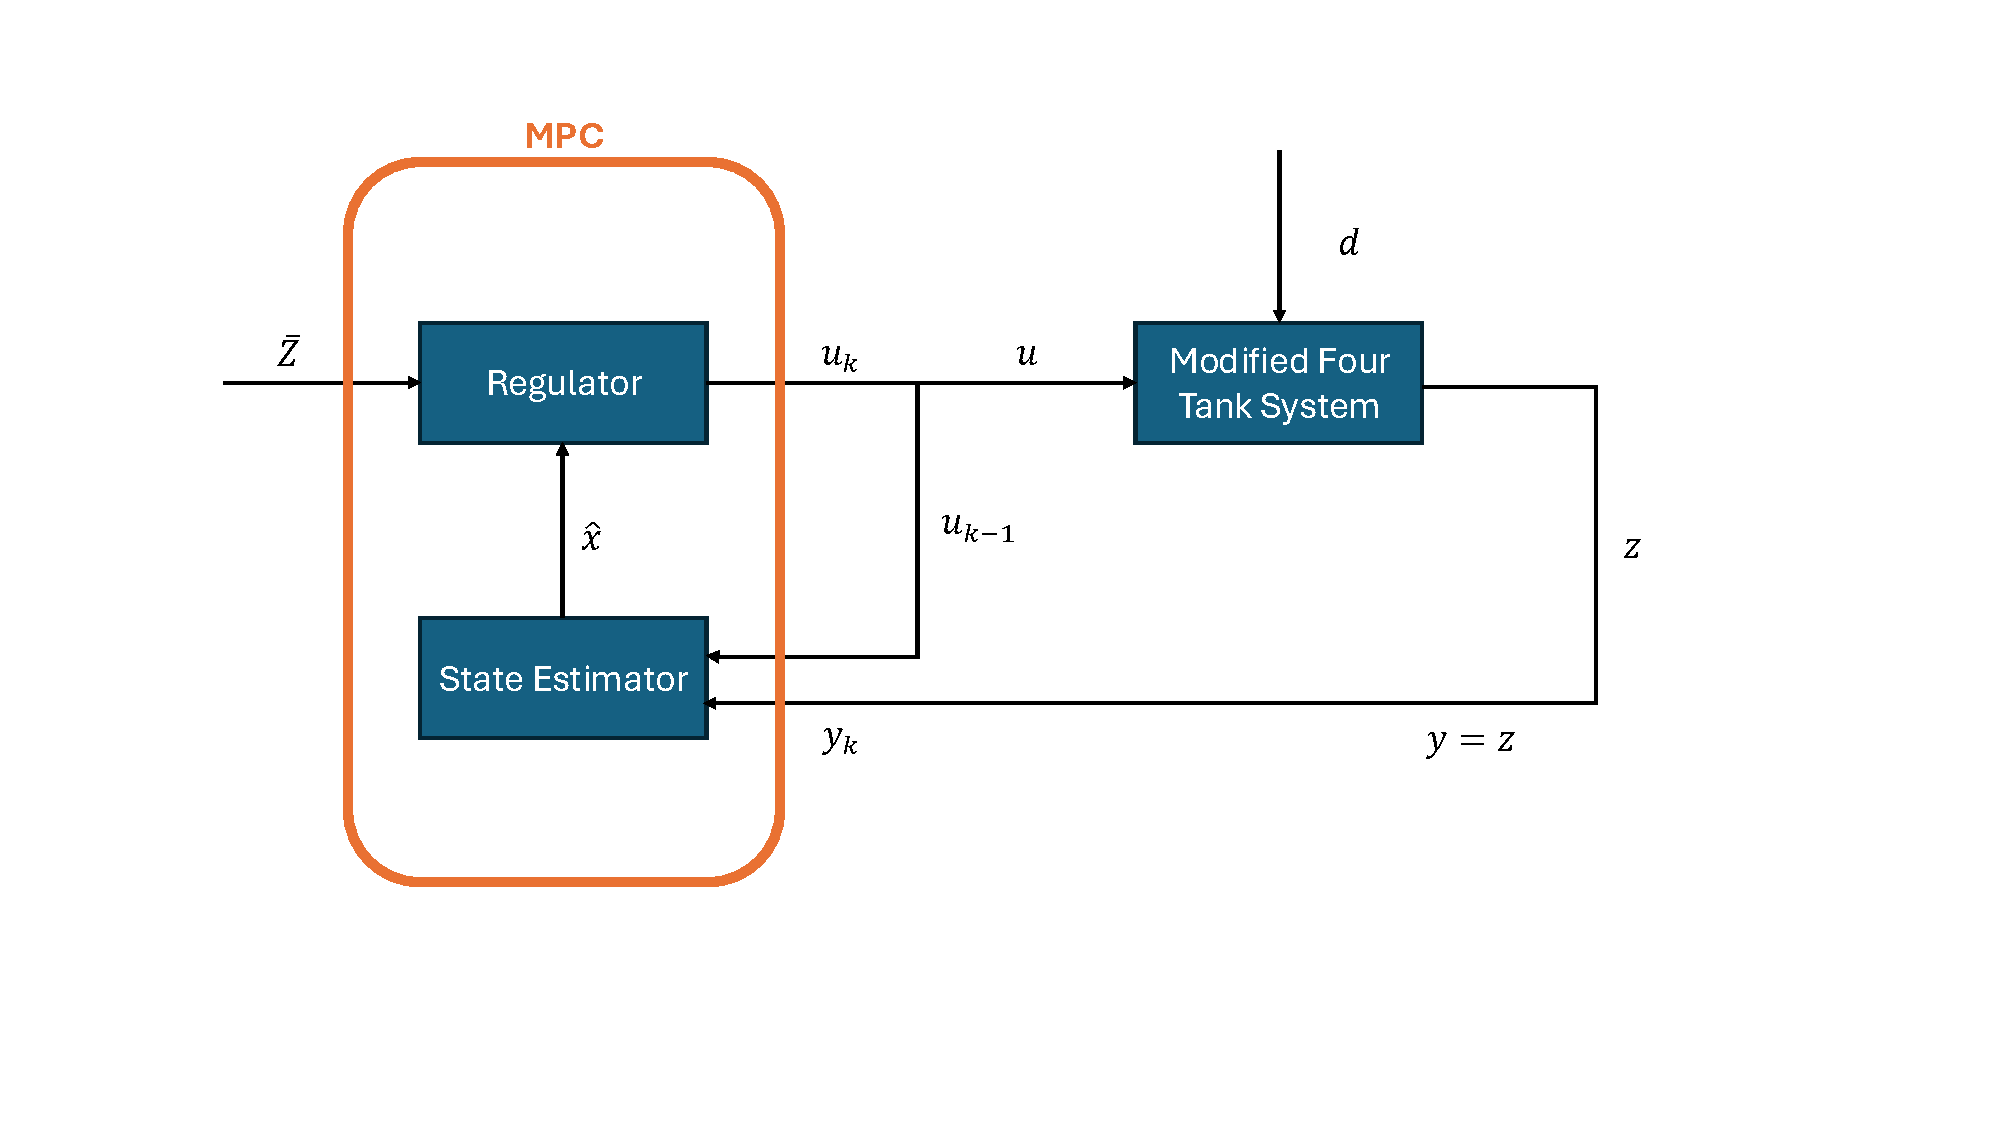
\includegraphics[width=0.8\linewidth]{figures/BlockDiagram.pdf}
     \caption{Block diagram of the Modified Four Tank System with a MPC system.}
     \label{fig:Blockdiagran}
 \end{figure}

 where $\overline{Z}$ is the setpoints for the levels in tank 1 and tank 2, $u_k$ is the manipulated flows $F_1$ and $F_2$ computed by the regulator at time $t_k$ while $u_{k-1}$ is the input used in the previous time interval $t_{k-1}$. The disturbance $d$ consists of the unmeasured flows $F_3$ and $F_4$. The controlled variable $z$ is the levels in tank 1 and tank 2 and since these are also the measured variables, the measurement is $y = z$, sampled as $y_k$ for the current time interval $t_k$. Lastly, $\hat{x}$ is the state estimate computed bu the state estimator and used as input for the regulator. 